\section{Timing Diagram}
Die Anforderungen aus den \glspl{Use-Case} \textbf{Boot.01} und \textbf{Poweroff.01}, die sich auf das Ein- und Ausschalten der Smartwatch beziehen, werden in den Abbildungen~\ref{fig:timing_diagram_power_on} und ~\ref{fig:timing_diagram_power_off} als Timing Diagrams dargestellt. Aus den \glspl{Requirement} geht hervor, dass sowohl das Einschalten als auch das Herunterfahren maximal 10 Sekunden dauern darf. Die Zeitmessung beginnt nachdem der entsprechende Vorgang durch das lange Drücken einer beliebigen Taste gestartet wurde.

\begin{figure}[h]
\centering\
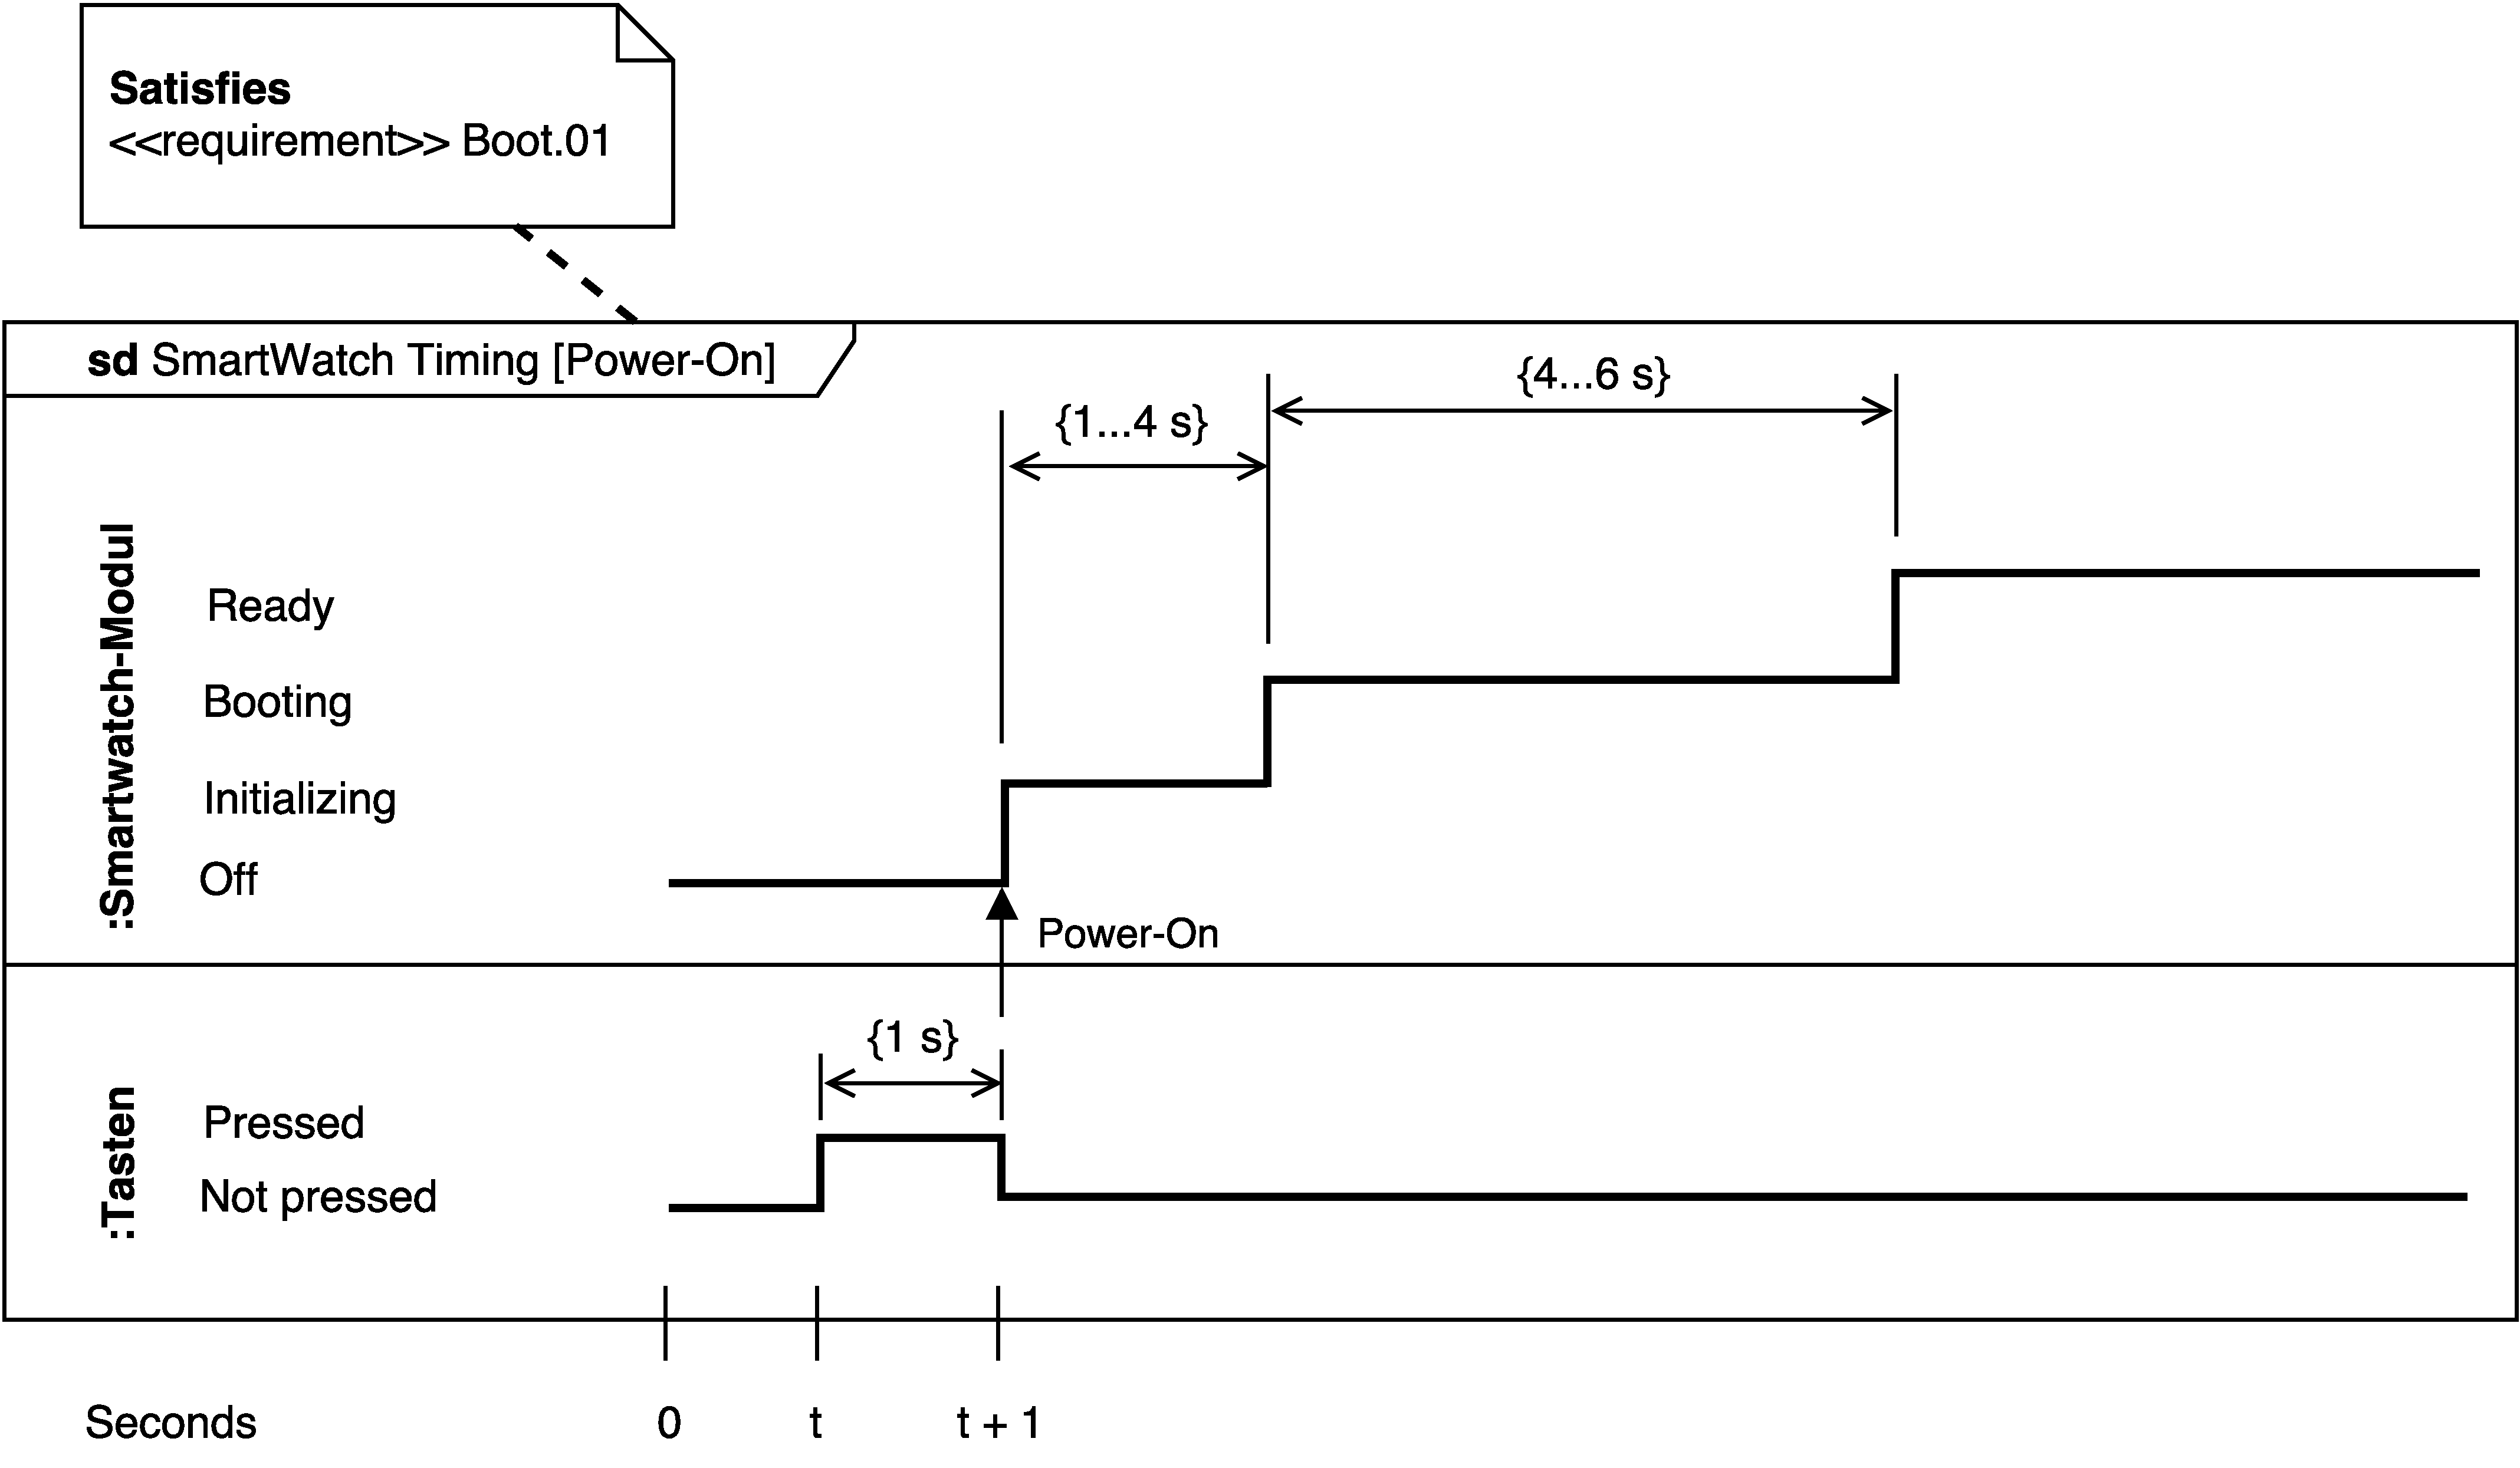
\includegraphics[width=14cm]{img/timing_diagram_power_on}
\caption[Timing Diagram: Power-On]{Darstellung des Startvorgangs der Smartwatch. Zur Verdeutlichung wird die \textit{Tasten}-Komponente seperat dargestellt}
\label{fig:timing_diagram_power_on}
\end{figure}

Um den einsekündigen Tastendruck zum Starten und den 5-sekündigen zum Ausschalten der Smartwatch zu verdeutlichen, wurde die \textit{Tasten}-Komponente in den Diagrammen separat dargestellt, obwohl sie eigentlich ein Bestandteil von \textit{Smartwatch-Modul} ist (siehe Abb.~\ref{fig:block2}).

\begin{figure}[h]
\centering\
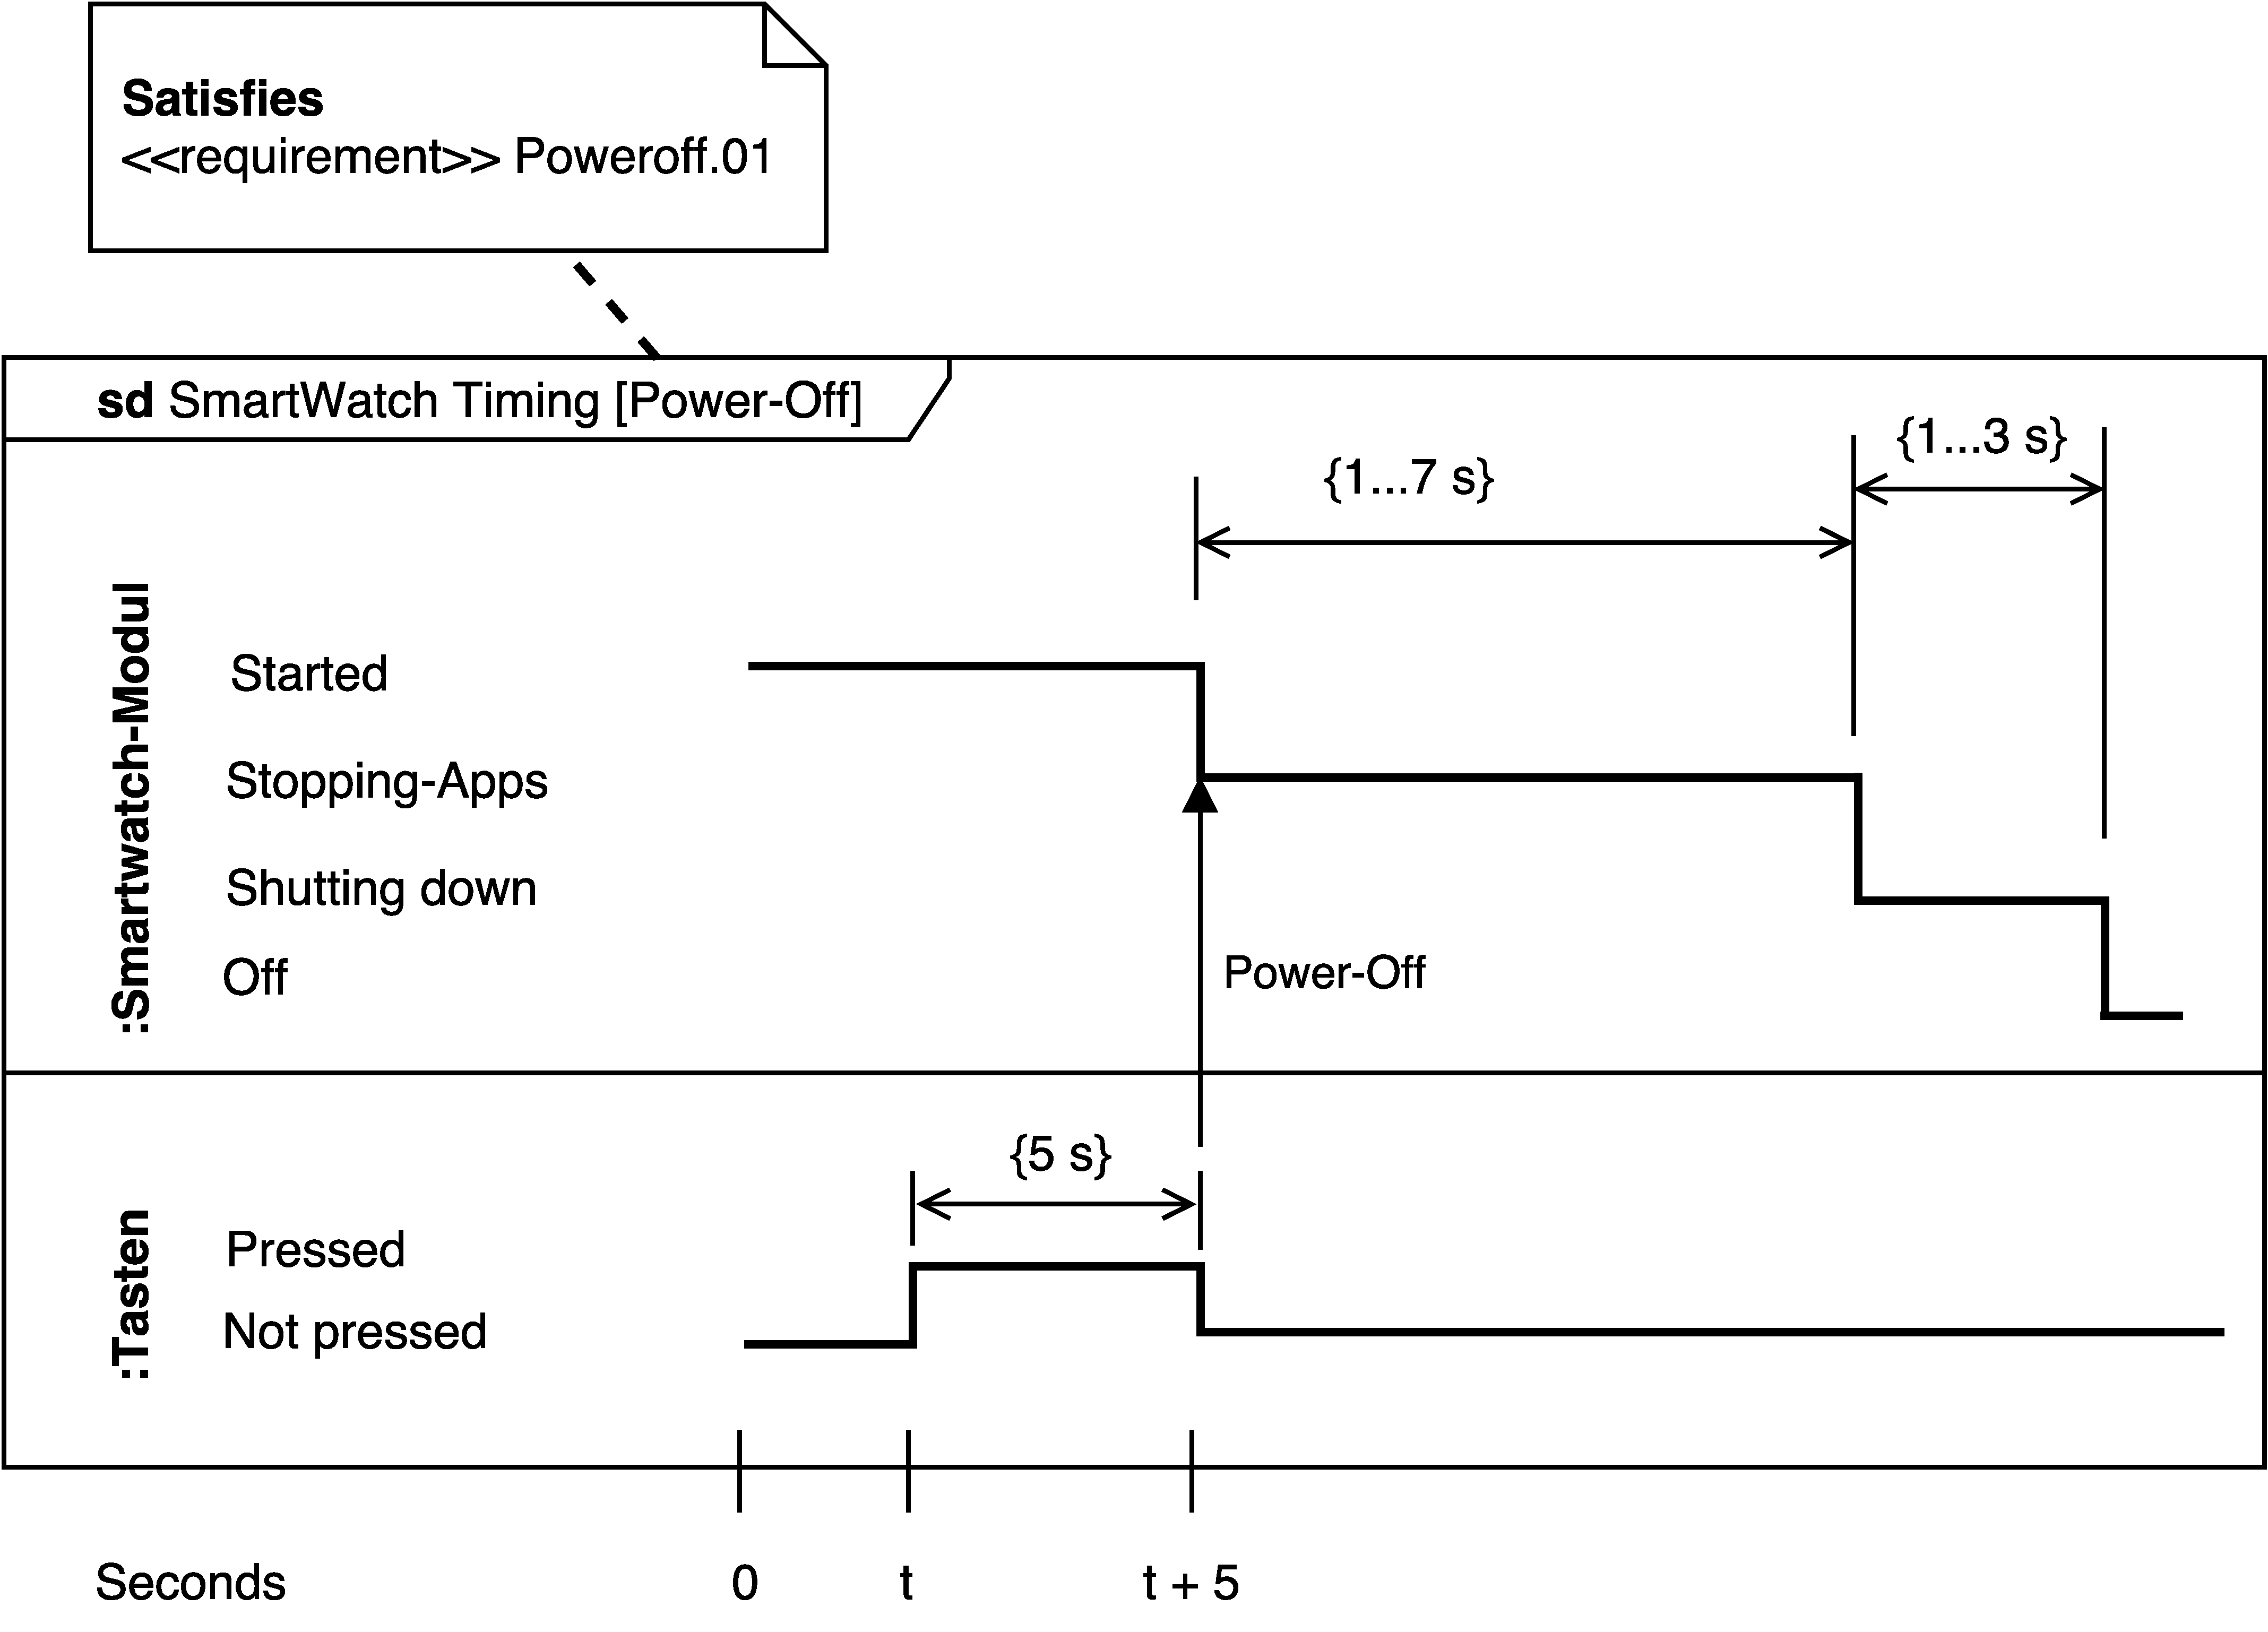
\includegraphics[width=14cm]{img/timing_diagram_power_off}
\caption[Timing Diagram: Power-Off]{Timing Diagram zur Verdeutlichung des Herunterfahrens der Smartwatch}
\label{fig:timing_diagram_power_off}
\end{figure}
